
Test afsnittet er opdelt i tre underafsnit. 
Først beskrives hvordan enhedstest er udført, derefter beskrives integrationstest og afslutningsvis beskrives accepttest. 

\chapter{Enhedstest}
I dette afsnit beskrives hvordan enhedstest af systemets enheder er udført. Enhedstesten bruges til at verificerer, at hver enkelt del virker uafhængigt af andre enheder. 
Der testes primært basal funktionalitet af enhederne, og i nogle tilfælde undersøges hvorvidt krav fra kravspecifikationen opfyldes.


\section{3G modul}

Enhedstest af 3G modulet foregår ved test af PUT og GET request, som er de metoder der er implementeret på dronen.

For udelukkende at have fokus på 3G modulet under enhedstesten, testes der ikke op imod den server som ellers anvendes til projektet. I stedet benyttes hjemmesiden requestb\footnote{requestb.in} , en hjemmeside der der tillader test af HTTP kommunikation. Ved at tilgå Requestb og starte en session tildeles en URL der kan bruges til test. Requestb indsamler information om alle HTTP request lavet til den tildelte URL. 

På figur \ref{fig:get_req} vises et GET request der sendes fra 3G modulet til en requestb.in server. Den første linje efter \textit{data:} fortæller om requestet er gennemført succesfuldt eller ej. Svaret \textit{200 ok} betyder at GET requestet er gået igennem og det ønskede data på korrekt vis er hentet. 

\vspace{0.3cm}

\begin{figure}[H]
\centering
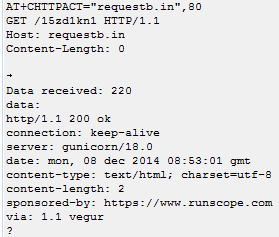
\includegraphics[width=0.5\textwidth]{Billeder/Test/get_requestbin.png}
\caption{GET Request}
\label{fig:get_req}
\end{figure}

\newpage

PUT request bruges til at sende data til eller opdatere information på server. 
På figur \ref{fig:putrequest_module} vises et PUT der sendes fra 3G modulet til requestb.in. De føreste seks linjer på figur \ref{fig:putrequest_module} viser requestet header med linje syv er requestet body. 

\begin{figure}[H]
\centering
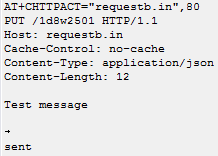
\includegraphics[width=0.5\textwidth]{Billeder/Test/putrequest_module.png}
\caption{PUT metode}
\label{fig:putrequest_module}
\end{figure}

\vspace{1cm}

På figur \ref{fig:put_req} vises det information der tilgængelig på server efter PUT requestet er fuldført. \textit{RAW BODY} viser det data der er modtaget og HEADERS indeholder parametrene for HTTP protokollen.

\begin{figure}[H]
\centering
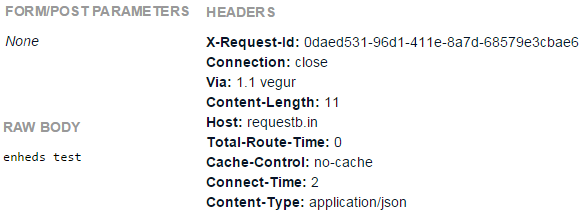
\includegraphics[width=0.8\textwidth]{Billeder/Test/put_request.png}
\caption{Information på server}
\label{fig:put_req}
\end{figure}



\newpage
\section{Afstandssensor}

I denne sektion beskrives hvordan ultralydssensoren HC-SR04 er testet for at fastslå hvor pålidelig den er. Testen er udført ved at lave gentagne målinger af afstand mellem ultralyds sensor og en væg. For hver deltest er der foretaget 100 målinger og maksimal værdi, minimal værdi og gennemsnit fundet. 

Ultralydssensoren bruges både til højdemåling og antikollison. Testen bruges til at kontrollere hvorvidt sensoren kan opfylde krav om nøjagtighed til højdemåling\footnote{Se ikke funktionelle krav i \textit{Kravspecifikation}}. 

Undervejs i testen ændres vinklen mellem ultralydssensor og væg, hvilket indirekte betyder afstande også ændres til væggen. I udgangspunkt skyder sensoren lyd ud i vandret retning og efterhånden ændres vinklen. Det formodes at sensoren fungerer bedst når der er en 90 graders vinkel mellem sensor og væg. 

På figur \ref{fig:ultra_testopstilling} vises en skitse af den anvendte testopstilling og tabellen nederst på siden viser resultater af den udførte test.

\begin{figure}[H]
\centering
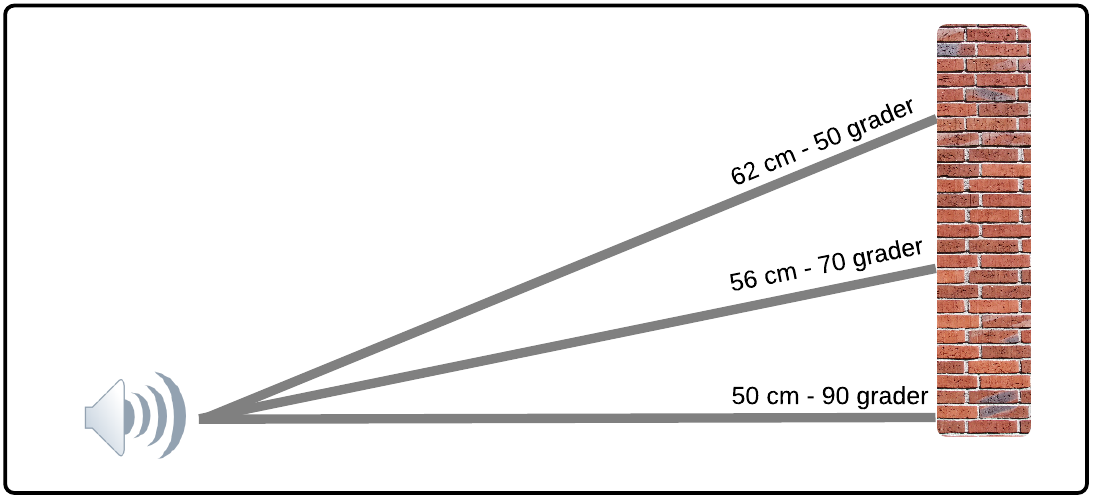
\includegraphics[width=1\textwidth]{Billeder/Test/ultrasound.png}
\caption{Skitse af testopstilling}
\label{fig:ultra_testopstilling}
\end{figure}

\vspace{0.5cm}

\begin{table}[H]
\begin{tabular}{| p{2.5cm}| p{2.5cm}| p{2.5cm}| p{2.5cm}| p{2.5cm}|}
\hline
\textbf{Vinkel} & \textbf{Afstand} & \textbf{Maks måling} & \textbf{Min måling}  & \textbf{Middel værdi} \\ \hline
0 & 50 cm & 49.0 cm & 48.0 cm  & 48.02 cm \\ \hline
20 & 56 cm & 49.0 cm & 49.0 cm  & 49.0 cm \\ \hline
40 & 62 cm & 50.0 cm & 51.0 cm  & 50.0 cm \\ \hline

\end{tabular}
\caption{Test ultralydssensor}
\label{tab:Ultralyds_test}
\end{table}




\newpage
\section{GPS}

Selvom GPSen sidder på 3G/GPS modulet kan det testes for sig selv. 

For at finde den eksakte GPS position fra GPS modulet, testes modulet i forskellige omgivelser. Som kontrol findes koordinaterne for den aktuelle position. Ud fra de fundne koordinater beregnes en afstand i meter, denne afstand fortæller lidt om afvigelsen af GPS modulet. I kravene er der defineret hvor stor en afvigelse GPS modulet må have. Denne afvigelse skal overholdes under tests, men da den aktuelle position har en afvigelse, vil afgivelsen i meter være påvirket. Denne påvirking vil føre til at afvigelsen i meter kan være større end de tilladte 2.5 meter som der er defineret i kravene.
Det har ikke været muligt at teste GPS modulet indendøre, da der ikke var GPS signal tilgængeligt. 

\begin{table}[H]
\begin{tabular}{| p{4cm}| p{4cm}| p{3cm}|}
\hline
GPS moduls koordinater & Aktuelle position & Afvigelse i meter\\\hline
Latitude:10.191518 \newline Longitude: 56.171863 & Latitude: 10.191560 \newline Longitude: 56.171896 & 4 meter\\\hline
Latitude: \newline Longitude & Latitude: \newline Longitude & \\\hline
Latitude: \newline Longitude & Latitude: \newline Longitude & \\\hline

\end{tabular}
\caption{GPS modul}
\label{tab:GPS_modul}
\end{table}



\newpage 
\section{PWM opsætning}

Testen bruges til at fastslå hvorvidt det PWM signal, der genereres af main controller, udsendes med korrekt frekvens og pulsbredde. Testen foregår ved at ændre værdien af compare-registeret\footnote{Se implementation view i \textit{Systemarkitektur og Design}} . Ændringer i compare registerets værdi bør medføre ændringer af pulsbredde i det PWM signal der udsendes fra main controller. 

Indledningsvis indstilles compare-registeret med værdi på 16000, derefter ændres værdien til 24000 og til sidst sættes compare-registerets værdi til 32000. Ved brug af oscilloskop kontrolleres om PWM signal har den korrekte pulsbredde. 

Nedenfor ses en tabel der viser hvordan testen forløb. Efter tabellen vises oscilloskop billeder taget under testen. 

\vspace{0.50cm}

\begin{table}[H]
	\centering
		\begin{tabular}{|c|c|c|c|}
			\hline
			Værdi compare reg. & Frekvens & Forventet pulsbredde & Faktisk pulsbredde \\ \hline
			16000 & 245 Hz & 1.00 ms & 1.00 ms \\ \hline			
			24000 & 245 Hz & 1.50 ms & 1.50 ms \\ \hline
			32000 & 245 Hz & 2.00 ms & 2.00 ms \\ \hline
		\end{tabular}
	\caption{Test resultat}
\end{table}

\vspace{0.50cm}

Figur \ref{fig:PWM_1} vises PWM signal hvor compare register har værdi på 16000. 

\begin{figure}[H]
\centering
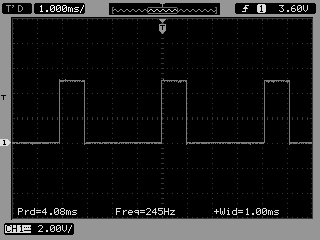
\includegraphics[width=0.7\textwidth]{Billeder/Test/PWM_16000.png}
\vspace{-0.0cm}
\caption{PWM signal - Compare register 16000}
\label{fig:PWM_1}
\end{figure}

\newpage

Figur \ref{fig:PWM_2} vises PWM signal hvor compare register har værdi på 24000. 
\begin{figure}[H]
\centering
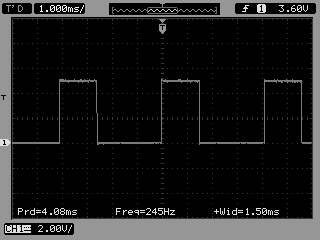
\includegraphics[width=0.7\textwidth]{Billeder/Test/PWM_24000.png}

\caption{PWM signal - Compare register 24000}
\label{fig:PWM_2}
\end{figure}

\vspace{0.5cm}

Figur \ref{fig:PWM_3} vises PWM signal hvor compare register har værdi på 32000. 
\begin{figure}[H]
\centering
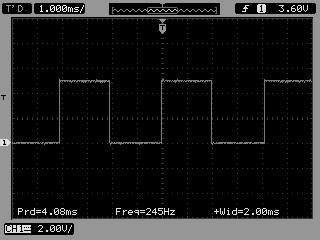
\includegraphics[width=0.7\textwidth]{Billeder/Test/PWM_32000.png}
\vspace{-0.0cm}
\caption{PWM signal - Compare register 32000}
\label{fig:PWM_3}
\end{figure}

%\newpage
%\section{Enhedstest software}
Til test af softwaren til systemet er enhedstests benyttet. Enhedstest er den test metode hvor softwaren deles op i mindst mulige dele og tests helt isolerede fra resten af systemet. Under enhedstest sikres at hver enhed i systemet fungere efter hensigten. Enhedstest bliver udarbejdet samtidig med produktions koden  bliver udviklet, på den måde bliver de fleste fejl i systemet fanget, mens systemet er under udvikling. Dvs fejl i systemet bliver opdaget samtidig med at systemet er under udvikling, hvilket mindsker fejlens omfang og omkostninger for at rette fejlen.

På figur \ref{fig:test_forlob} ses mængende af fejl i div testforløb og fokus opdelningen.
\begin{figure}[H]
	\centering
	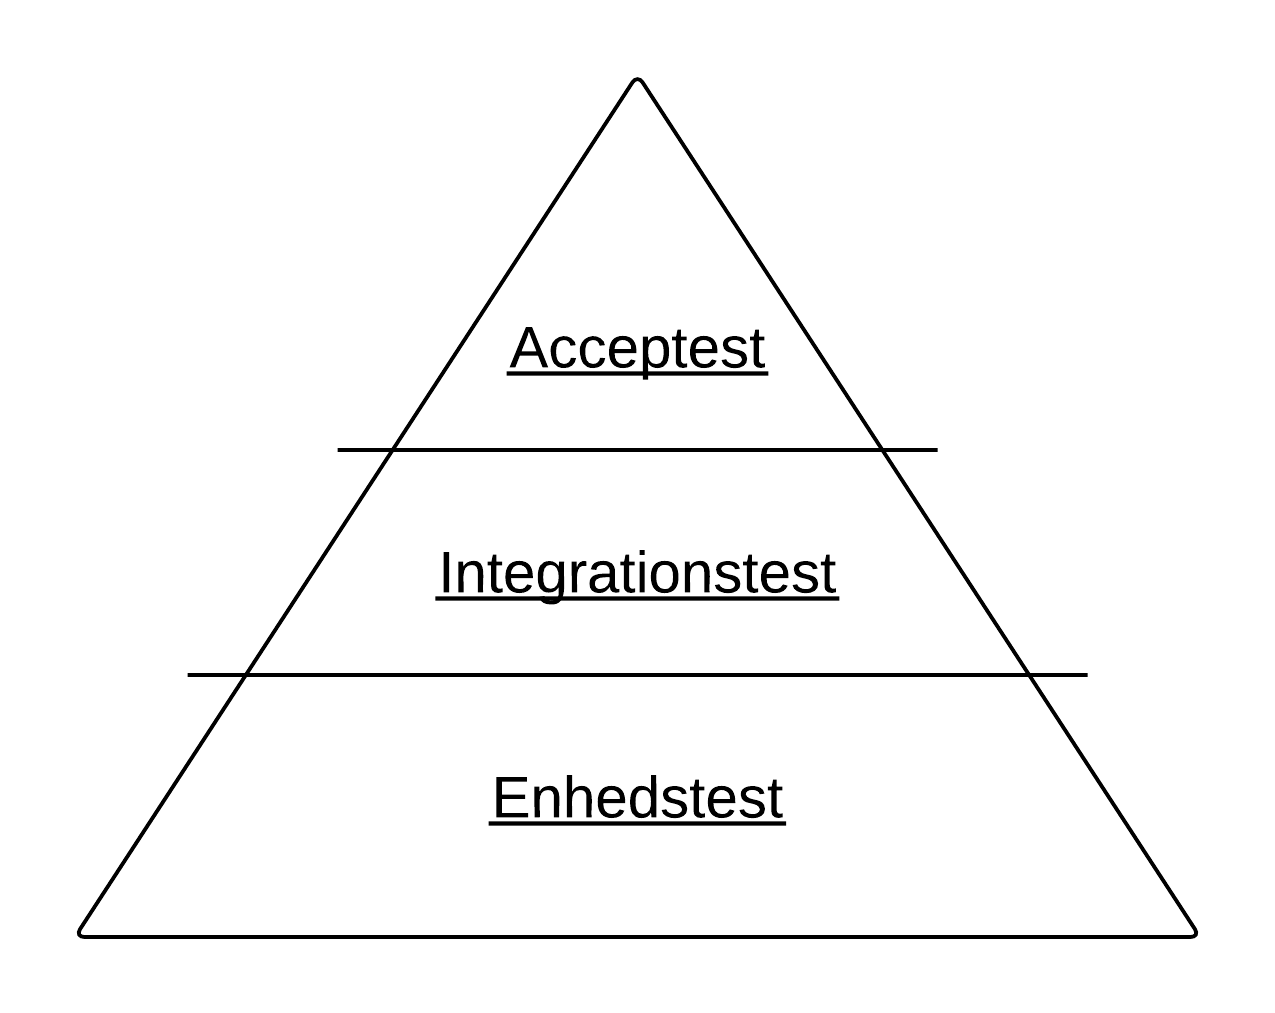
\includegraphics[width=0.6\textwidth]{Billeder/Test/forlob.png}
	\caption{Mængden af fejl}
	\label{fig:test_forlob}
\end{figure}

\subsection{Test opbygning}
Enhedstestene er opbygget efter AAA-modellen\footnote{http://c2.com/cgi/wiki?ArrangeActAssert}.\\ 
Arrange: \\
Her opsættes input til testen, eller evt afhængigheder håndteres. \\
Act: \\
Her bliver det ønskede kode stimuleret. \\
Assert: \\
Her forventes et bestemt output og testen afgøres om den er succesfuld eller ej.

\newpage
På  figur \ref{fig:aaa} ses et eksempel på AAA modellen. I testen bliver der testet for om den korrekte metode bliver kaldt når bruger prøver at logge in på webapplikationen. 

\begin{figure}[H]
	\centering
	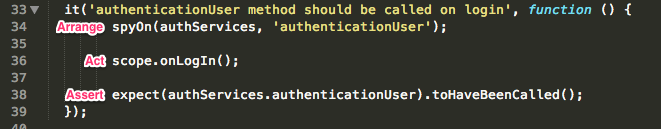
\includegraphics[width=0.6\textwidth]{Billeder/Test/aaa.png}
	\caption{AAA eksempel}
	\label{fig:aaa}
\end{figure}

\newpage
\input{Kapitler/Test/Webapplikation}


I dette afsnit beskrives hvordan enhedstest af systemets moduler er udført. Der testes primært basal funktionalitet af modulerne, og i nogle tilfælde undersøges hvorvidt krav fra kravspecifikationen opfyldes. I afsnittet testes blandt andet præcision af GPS og højdemåler.


\subsection{PWM opsætning}

Testen bruges til at fastslå hvorvidt det PWM signal der genereres af main controller udsendes med korrekt frekvens og pulsbredde. Testen foregår ved at ændre værdien af compare-registeret \footnote{Se implementation view i \textit{Systemarkitektur og Design}} . Ændringer i compare registerets værdi bør medføre ændringer af pulsbredde i det PWM signal der udsendes fra main controller. 

Indledningsvis indstilles compare-registeret med værdi på 16000, derefter ændres værdien til 24000 og til sidst sættes compare-registerets værdi til 32000. Ved brug af oscilloskop kontrolleres om PWM signal har den korrekte pulsbredde. 

Nedenfor ses en tabel der viser hvordan testen forløb. Efter tabellen vises oscilloskop billeder taget under testen. 

\vspace{0.50cm}

\begin{table}[H]
	\centering
		\begin{tabular}{|c|c|c|c|}
			\hline
			Værdi compare reg. & Frekvens & Forventet pulsbredde & Faktisk pulsbredde \\ \hline
			16000 & 245 Hz & 1.00 ms & 1.00 ms \\ \hline			
			24000 & 245 Hz & 1.50 ms & 1.50 ms \\ \hline
			32000 & 245 Hz & 2.00 ms & 2.00 ms \\ \hline
		\end{tabular}
	\caption{Test resultat}
\end{table}

\vspace{0.50cm}

Figur \ref{fig:PWM_1} vises PWM signal hvor compare register har værdi på 16000. 

\begin{figure}[H]
\centering
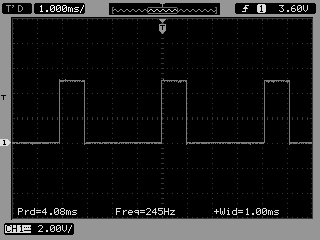
\includegraphics[width=0.7\textwidth]{Billeder/Test/PWM_16000.png}
\vspace{-0.0cm}
\caption{PWM signal - Compare register 16000}
\label{fig:PWM_1}
\end{figure}

\newpage

Figur \ref{fig:PWM_2} vises PWM signal hvor compare register har værdi på 24000. 
\begin{figure}[H]
\centering
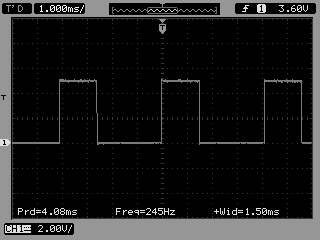
\includegraphics[width=0.7\textwidth]{Billeder/Test/PWM_24000.png}

\caption{PWM signal - Compare register 24000}
\label{fig:PWM_2}
\end{figure}

\vspace{0.5cm}

Figur \ref{fig:PWM_3} vises PWM signal hvor compare register har værdi på 32000. 
\begin{figure}[H]
\centering
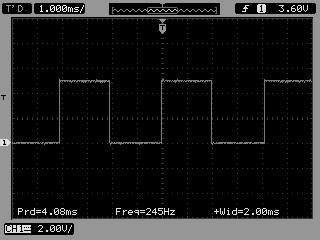
\includegraphics[width=0.7\textwidth]{Billeder/Test/PWM_32000.png}
\vspace{-0.0cm}
\caption{PWM signal - Compare register 32000}
\label{fig:PWM_3}
\end{figure}



 

\chapter{Integrationstest}

\section{Kommunikation mellem drone og server}

Dette afsnit beskriver testen af kommunikationen mellem drone og server. 

Kommunikationen er testet ved at bruge 3G modulet på drone som benytter HTTP protokollens GET og PUT metoder. 
Idet serveren er en passiv enhed, er det 3G modulet der skal tage initiativet til at hente eller sende data. 

På figur \ref{fig:integrationstest_webserver} vises hvordan informationen på serveren ser ud. Ved brug af et GET request ønskes disse information hentet ned: 

\begin{figure}[H]
\centering
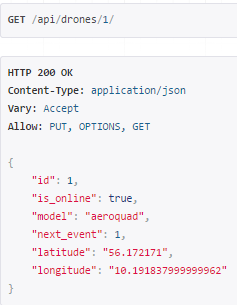
\includegraphics[width=0.4\textwidth]{Billeder/Test/integratest_webserver.png}
\caption{Webserver UI}
\label{fig:integrationstest_webserver}
\end{figure}

Ved brug af GET metoden på serverens URL (iha-11726.iha.dk/api/drones/1/), får 3G modulet informationen på figur \ref{fig:getfromserver} returneret. Dette information deles op i en header og body, hvor headeren kasseres og body sorteres ved hjælp af et JSon bibliotek.

\begin{figure}[H]
\centering
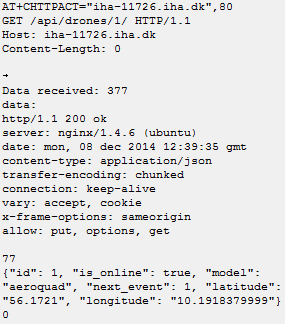
\includegraphics[width=0.4\textwidth]{Billeder/Test/getfromserver.png}
\caption{GET data fra server}
\label{fig:getfromserver}
\end{figure}

Ved brug af PUT metoden, skal der sendes et request til serveren. Dette request skal indeholde serverens URL og de informationer der ønskes sendt. Et request der er brugt af 3G modulet ser ud som på figur \ref{fig:puttoserver}.

\begin{figure}[H]
\centering
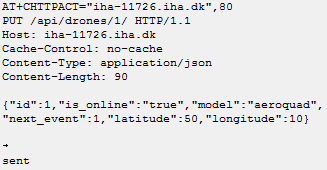
\includegraphics[width=0.5\textwidth]{Billeder/Test/put_dronerequest.png}
\caption{PUT request til server}
\label{fig:puttoserver}
\end{figure}

 Ved at sende den viste string, opdateres informationerne på serveren. På figur \ref{fig:putdata_server} vises det opdaterede information på serveren.
 
 \begin{figure}[H]
\centering
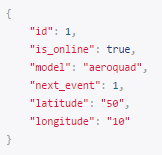
\includegraphics[width=0.4\textwidth]{Billeder/Test/putdata_server.png}
\caption{PUT fra server}
\label{fig:putdata_server}
\end{figure}

\newpage
\section{Drone Flight Control}
\subsection{Flyvehøjde}

Dette afsnit beskriver test af tilpasning af flyvehøjde.

For at dronen ved hvilken højde den skal flyve i, skal flyveopsætningen være hentet fra serveren. Når flyvehøjden og de ønskede GPS positioner er kendt, begynder dronen at lette. Main controlleren anvender højdesensorer til at finde højden med. Så længe at højden ikke er indenfor det ønskede interval, skal den hæve eller sænke sin højde, det gør den ved enten at forøge eller formindske throttle. 

På figur \ref{fig:skift_hoejde} ses hvad der sker, hvis højden enten er for høj eller for lav. Først måles den aktuelle højde, denne sammenlignes med minimumshøjden og den maksimalehøjde, hvis den er udenfor det interval reguleres der på throttle. 

\begin{figure}[H]
\centering
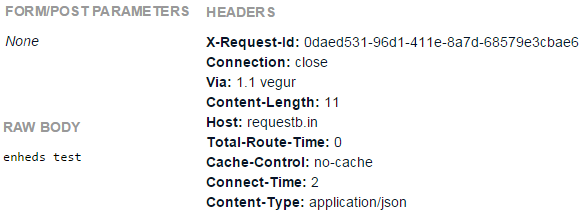
\includegraphics[width=0.8\textwidth]{Billeder/Test/put_request.png}
\caption{Tilpasning af højde}
\label{fig:skift_hoejde}
\end{figure}
\newpage

\section{Tilpas orientering}

Dette afsnit beskriver test af dronens orientering. Dronen skal have den rette orientere, før den kan flyve fremad. For at finde orienteringen, bruges 3G/GPS modulet, kompas og main controlleren.

Til testen af orientering er nuværende og ønskede GPS positioner hardcoded. 
Den nuværende og ønskede GPS positions sammenlignes og orienteringen findes. 
Fra kompasset aflæser main controlleren dronens orientering og sammenligner med den ønskede orientering. Hvis orienteringerne ikke ligger indenfor det ønskede interval, skal dronen ændre retning. Dronens flyveretning ændres ved kortvarigt at forøge Yaw parameteren. 


På figur \ref{fig:orientering_skift} vises hvad main controlleren gør. Main controlleren sammenligner nuværende orientering med ønskede orientering, hvis orienteringen ikke er indenfor det ønskede interval, ændres denne ved ændre på indstillingen af Yaw.

\begin{figure}[H]
\centering
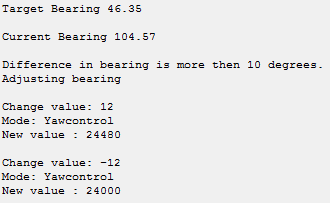
\includegraphics[width=0.5\textwidth]{Billeder/Test/bearing_test.png}
\caption{Ændring af orientering}
\label{fig:orientering_skift}
\end{figure}

\vspace{0.5cm}

Hvis orienteringen er indenfor intervallet, vil outputtet være som på figur \ref{fig:orientering_interval}.

\begin{figure}[H]
\centering
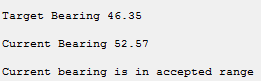
\includegraphics[width=0.4\textwidth]{Billeder/Test/bearing_reached.png}
\caption{Orientering er i intervallet}
\label{fig:orientering_interval}
\end{figure}
\newpage

\chapter{Accepttest \\ Funktionelle krav}

\vspace{-1cm}

\section*{Formål}
\vspace{-0.5cm}

Dette afsnit specificerer accepttest af systemets funktionelle krav. 

Hvis der under accepttesten opstår fejl, der umuliggør fortsat test af efterfølgende testcases afbrydes denne test. Hvis der opstår fejl i enkelte testcases, men fortsat accepttest er mulig, underkendes den enkelte test og accepttesten fortsættes.

Såfremt en test afbrydes, underkendes eller ikke kan gennemføres, angives den eller de step der ikke kan gennemføres i kapitlet \textbf{Fejl og mangler}. 


\section*{Testspecifikation}
\vspace{-0.5cm}
Software der skal testes:
\begin{table}[H]
	\centering
		\begin{tabular}{|c|c|c|c|}
			\hline
			Software & Version & Release dato & Bemærkning \\ \hline
			Server & Rev. 226b85b & 23/11-2014 & \\ \hline			
			Webapplikation & Rev. 7969aac & 04/12-2014 &\\ \hline
		\end{tabular}
	\caption{Software til test}
\end{table}

Hardware der skal testes:
\begin{table}[H]
	\centering
		\begin{tabular}{|c|c|c|c|}
			\hline
			Hardware & Version & Release dato & Bemærkning \\ \hline
			Kompas 			& Rev. 9d3ec7b & 17/11-2014 &  \\ \hline			
			Højdemåler 		& Rev. 9d3ec7b & 17/11/2014 &  \\ \hline
			3G/GPS modul 	& Rev. 51ec5ac & 7/11-2014 &  \\ \hline
			Switch board 	& Rev. 9d3ec7b & 17/11/2014 &  \\ \hline
		\end{tabular}
	\caption{Hardware til test}
\end{table}

\vspace{-0.5cm}
\section*{Testprocedure}
\vspace{-0.5cm}
De individuelle use cases og scenarier i kravspecifikationen testes i enkelte test cases. 

\begin{itemize}
	\item Hvis et teststep gennemføres fejlfrit markeres dette med ”Godkendt” i feltet ”resultat” for det pågældende test step.

	\item Hvis et teststep gennemføres med ubetydelige fejl, markeres dette med ”(OK)” i feltet ”resultat” for det pågældende test step.
	
	\item Hvis et teststep ikke kan gennemføres eller gennemføres med betydelige fejl, markeres dette med "Ikke godkendt".
	
\end{itemize}

\newpage

\section{Test case 1: Start drone}
Use case under test: UC 1: Start drone.\\
Forudsætninger:	Ingen.

\textbf{Hovedscenarie}
\begin{table}[H]
	\centering
		\begin{tabular}{|l|p{5 cm}|p{5 cm}|p{2.5 cm}|} 
		\hline
			\textbf{Step} & \textbf{Handling} & \textbf{Forventet resultat} & \textbf{Resultat} \\ \hline
			1 & Bruger tilslutter batteri og dronen tændes. & Systemet tilføres forsyning og ESC'er signalerer de er \newline forbundet til forsyning. & Godkendt.   \\ \hline
			2 & Main controller initialiseres. & Main controller startes. & Godkendt.   \\ \hline
			3 & GPS initialiseres og dronens nuværende GPS position \newline opdateres. & Nuværende GPS position \newline opdateres og gemmes lokalt på main controller. & Godkendt.   \\ \hline
			4 & 3G initialiseres og dronen opretter forbindelse til \newline 3G-netværket. & Dronen tilsluttes det mobile \newline 3G-netværk. &  Godkendt. \\ \hline
			5 & Dronens nuværende GPS \newline position sendes til server. & På webapplikation vises \newline drones nuværende position og at dronen er online. & Godkendt. \\ \hline
		\end{tabular}
\end{table}

\textbf{Extension 1: Forbindelse kan ikke oprettes.}
\begin{table}[H]
	\centering
		\begin{tabular}{|l|p{5 cm}|p{5 cm}|p{2.5 cm}|} 
		\hline
			\textbf{Step} & \textbf{Handling} & \textbf{Forventet resultat} & \textbf{Resultat} \\ \hline
			a & Systemet indikerer fejl og bruger genstarter systemet. & Systemet genstartes og \newline forbindelse oprettes. & Ikke Godkendt. \\ \hline
		\end{tabular}
\end{table}

\newpage
\section{Test case 2: Ny flyveopsætning}
Use case under test: UC 2: Ny flyveopsætning.\\
Forudsætninger:	Bruger er oprettet i systemet og UC\#1 er succesfuld gennemført.

\textbf{Hovedscenarie}
\begin{table}[H]
	\centering
		\begin{tabular}{|l|p{5 cm}|p{5 cm}|p{2.5 cm}|}
		\hline
			\textbf{Step} & \textbf{Handling} & \textbf{Forventet resultat} & \textbf{Resultat} \\ \hline
			1 & Bruger logger på \newline webapplikation. & Login lykkes, og webapplikationens forside vises. & Godkendt. \\ \hline
			2 & Fra forsiden navigerer bruger til flyveopsætning. & Flyveopsætnings siden vises. & Godkendt. \\ \hline
			3 & Bruger laver en ny \newline flyveopsætning og vælger: \newline
				- GPS lokationer der \newline skal flyves til. \newline
				- Om der skal tages billeder ved de valgte lokationer. \newline
				- Højde billeder skal tages fra. \newline
				- Generel flyvehøjde.				
				 & Flyveopsætning klargjort & (OK). \\ \hline
			4 & Bruger gemmer flyveopsætning og gør den tilgængelig på server. & Flyveopsætning gøres \newline tilgængelig på server & Ikke godkendt. \\ \hline
		\end{tabular}
\end{table}

\textbf{Extension 1: Fejl i login.}
\begin{table}[H]
	\centering
		\begin{tabular}{|l|p{5 cm}|p{5 cm}|p{2.5 cm}|} 
		\hline
			\textbf{Step} & \textbf{Handling} & \textbf{Forventet resultat} & \textbf{Resultat} \\ \hline
			a & Bruger føres tilbage til login. & Login kan påny forsøges. & Godkendt. \\ \hline
		\end{tabular}
\end{table}

\textbf{Extension 2: Der laves ikke ny flyveopsætning.}
\begin{table}[H]
	\centering
		\begin{tabular}{|l|p{5 cm}|p{5 cm}|p{2.5 cm}|} 
		\hline
			\textbf{Step} & \textbf{Handling} & \textbf{Forventet resultat} & \textbf{Resultat} \\ \hline
			a & Gemt flyveopsætning bruges. & Flyveopsætning klargjort. & Ikke godkendt.\\ \hline
		\end{tabular}
\end{table}

\newpage

\section{Test case 3: Flyv til position}
Use case under test: UC 3: Flyv til position.\\
Forudsætninger:	UC\#1 og UC\#2 er succesfuld gennemført.

\textbf{Hovedscenarie}
\begin{table}[H]
	\centering
		\begin{tabular}{|l|p{5 cm}|p{5 cm}|p{2.5 cm}|} 
		\hline
			\textbf{Step} & \textbf{Handling} & \textbf{Forventet resultat} & \textbf{Resultat} \\ \hline
			1 & Drone henter flyveopsætning fra server. & Der oprettes forbindelse \newline mellem server og drone \newline og flyveopsætning sendes. & Godkendt. \\ \hline
			2 & Nuværende position \newline opdateres. & Ingen handling  &  Godkendt. \\ \hline
			3 & Flyvehøjde tilpasses. & Flyvehøjde justeres & (OK). \\ \hline
			4 & Flyveorientering tilpasses. & Orientering justeres & Ikke godkendt. \\ \hline
			5 & Drone flyver mod \newline ønsket position. & Drone nærmer sig \newline ønsket position  &  Ikke godkendt. \\ \hline
			6 & Ønsket position er nået. & Ønsket position er nået. & Ikke godkendt. \\ \hline
		\end{tabular}
\end{table}

\textbf{Extension 1: Dronen henter ikke flyveopsætning.}
\begin{table}[H]
	\centering
		\begin{tabular}{|l|p{5 cm}|p{5 cm}|p{2.5 cm}|}
		\hline
			\textbf{Step} & \textbf{Handling} & \textbf{Forventet resultat} & \textbf{Resultat} \\ \hline
			a & Flyvning med en anden flyveopsætning er aktiv. & UC \#3 fortsættes med den aktive flyveopsætning. & Godkendt. \\ \hline
		\end{tabular}
\end{table}

\textbf{Extension 2: Ugyldig GPS koordinat.}
\begin{table}[H]
	\centering
		\begin{tabular}{|l|p{5 cm}|p{5 cm}|p{2.5 cm}|} 
		\hline
			\textbf{Step} & \textbf{Handling} & \textbf{Forventet resultat} & \textbf{Resultat} \\ \hline
			a & Drone går i fejlmode \#1. & Forsøger at finde gyldig GPS koordinat, mislykkes dette lander dronen. & Ikke godkendt.\\ \hline
		\end{tabular}
\end{table}

\textbf{Extension 3: Ugyldig flyvehøjde.}
\begin{table}[H]
	\centering
		\begin{tabular}{|l|p{5 cm}|p{5 cm}|p{2.5 cm}|}
		\hline
			\textbf{Step} & \textbf{Handling} & \textbf{Forventet resultat} & \textbf{Resultat} \\ \hline
			a & Drone går i fejlmode \#2. & Forsøger at finde gyldig \newline flyvehøjde, mislykkes dette lander dronen. & Ikke godkendt. \\ \hline
		\end{tabular}
\end{table}

\newpage

\section{Test case 4: Billede af position}
Use case under test: UC 4: Billede af position.\\
Forudsætninger:	UC\#3 er succesfuld gennemført.

\textbf{Hovedscenarie}
\begin{table}[H]
	\centering
		\begin{tabular}{|l|p{5 cm}|p{5 cm}|p{2.5 cm}|} 
		\hline
			\textbf{Step} & \textbf{Handling} & \textbf{Forventet resultat} & \textbf{Resultat} \\ \hline
			1 & Drone tager et billede af \newline nuværende position. & Kamera aktiveres og der \newline tages et billede. & Ikke godkendt. \\ \hline
			2 & Billedet sendes til server. & Billedet sendes til server gøres tilgængelig på \newline webapplikationen & Ikke godkendt. \\ \hline
			3 & Bruger giver accept af billedet via webapplikation. & Billedet gemmes i database  & Ikke godkendt. \\ \hline

		\end{tabular}
\end{table}


\textbf{Extension 1: Bruger beder om nyt billede.}
\begin{table}[H]
	\centering
		\begin{tabular}{|l|p{5 cm}|p{5 cm}|p{2.5 cm}|} 
		\hline
			\textbf{Step} & \textbf{Handling} & \textbf{Forventet resultat} & \textbf{Resultat} \\ \hline
			a & Drone instrueres til at \newline ændre flyvehøjde, orientering eller position. &  Flyvehøjde, orientering eller position ændres. & Ikke godkendt. \\ \hline
		\end{tabular}
\end{table}

\textbf{Extension 2: Bruger svarer ikke inden for tidsgrænsen.}
\begin{table}[H]
	\centering
		\begin{tabular}{|l|p{5 cm}|p{5 cm}|p{2.5 cm}|} 
		\hline
			\textbf{Step} & \textbf{Handling} & \textbf{Forventet resultat} & \textbf{Resultat} \\ \hline
			a & Drone får automatisk tildelt accept. & Drone påbegynder flyvning mod næste GPS lokation. & Ikke godkendt. \\ \hline
		\end{tabular}
\end{table}

\newpage
\section{Test case 5: Vis tidligere flyvning}
Use case under test: UC 5: Vis tidligere flyvning.\\
Forudsætninger:	Bruger er oprettet i systemet.

\textbf{Hovedscenarie}
\begin{table}[H]
	\centering
		\begin{tabular}{|l|p{5 cm}|p{5 cm}|p{2.5 cm}|} 
		\hline
			\textbf{Step} & \textbf{Handling} & \textbf{Forventet resultat} & \textbf{Resultat} \\ \hline
			1 & Bruger logger på \newline webapplikation. & Login lykkes og webapplikations forside vises. & Godkendt.  \\ \hline
			2 & Fra forsiden navigerer \newline bruger til historik. & En oversigt over tidligere \newline flyvninger vises. & Ikke godkendt. \\ \hline
			3 & Bruger vælger en specifik \newline tidligere flyvning. &  Billeder, video og flyverute \newline tilhørende valgte flyvning \newline vises. &  Ikke godkendt. \\ \hline			
		\end{tabular}
\end{table}

\textbf{Extension 1: Fejl i login.}
\begin{table}[H]
	\centering
		\begin{tabular}{|l|p{5 cm}|p{5 cm}|p{2.5 cm}|} 
		\hline
			\textbf{Step} & \textbf{Handling} & \textbf{Forventet resultat} & \textbf{Resultat} \\ \hline
			a & Bruger føres tilbage til login. & Login kan påny forsøges. & Godkendt. \\ \hline
		\end{tabular}
\end{table}

\section{Test case 6: Anti kollision}
Use case under test: UC 6: Anti kollision.\\
Forudsætninger:	UC\#3 er igangværende.

\textbf{Hovedscenarie}
\begin{table}[H]
	\centering
		\begin{tabular}{|l|p{5 cm}|p{5 cm}|p{2.5 cm}|} 
		\hline
			\textbf{Step} & \textbf{Handling} & \textbf{Forventet resultat} & \textbf{Resultat} \\ \hline
			1 & Anti kollisions system \newline detekterer en forhindring. & Bremser dronens fremdrift. & Ikke godkendt. \\ \hline
			2 & Undvigelsesmanøvre udføres. & Drone passere forhindring og flyver videre. & Ikke godkendt.\\ \hline			
		\end{tabular}
\end{table}

\textbf{Extension 1: Forhindringen kan ikke undviges.}
\begin{table}[H]
	\centering
		\begin{tabular}{|l|p{5 cm}|p{5 cm}|p{2.5 cm}|} 
		\hline
			\textbf{Step} & \textbf{Handling} & \textbf{Forventet resultat} & \textbf{Resultat} \\ \hline
			a & Drone går i fejlmode \#3. & Forsøger at finde måde at passere forhindring. Mislykkes det lander dronen. & Ikke godkendt. \\ \hline
		\end{tabular}
\end{table}




\chapter{Ikke funktionelle krav}

    \centering
    \begin{tabular}{|p{1. cm}|p{3.2 cm}|p{3.2 cm}|p{3.2 cm}|p{2.2 cm}|}
			\hline
			\multicolumn{5}{|l|}{\textbf{{\large Generelle krav}}}\\ \hline
			\textbf{Krav nr.} & \textbf{Krav} & \textbf{Test} & \textbf{Forventet \newline resultat} & 			
			\textbf{Godkend \& \newline kommentar} \\ \hline
			
			1.1 & Kommunikation mellem drone og webapplikation skal foregå trådløst.
				& Opsætning sendes til drone via webapplikation.
				& Den sendte opsætning modtages.
				& \\ \hline

			1.2 & Trådløs kommunikation benytter 3G protokol eller ældre. 
				& Der undersøges hvilken slags mobilnet 3G-modul er forbundet til.
				& Det verificeres at protokollen passer.
				&  \\ \hline
			
			1.3 & Ultralyds sensor skal måle højde $\pm$ 10 cm.
				& Ultralyds sensor placeres i en kendt afstand til en væg.
				& Afstanden måles med korrekt længde.
				& \\ \hline						
		\end{tabular}

\vspace{2cm}

    \centering
    \begin{tabular}{|p{1. cm}|p{3.2 cm}|p{3.2 cm}|p{3.2 cm}|p{2.2 cm}|}
			\hline
			\multicolumn{5}{|l|}{\textbf{{\large Krav til webapplikation}}}\\ \hline
			\textbf{Krav nr.} & \textbf{Krav} & \textbf{Test} & \textbf{Forventet \newline resultat} & 			
			\textbf{Godkend \& \newline kommentar} \\ \hline
			
			2.1 & Webapplikation skal kunne tilgås via både computere og telefoner.
				& Webapplikationen tilgås på både computer og telefon.
				& Applikationen tilpasser sig til den forbundne enhed.
				& \\ \hline

			2.2 & Indholder database med billeder og flyveruter fra tidligere. 
				& Databasen tilgås, billeder og flyveruter vises.
				& Databasen indeholder billeder og flyveruter.
				&  \\ \hline
			
			2.3 & Indholder database med brugere.
				& Webapplikation tilgås og det verificeres at bruger kan logge ind.
				& Bruger kan logge på webapplikation.
				& \\ \hline				
		\end{tabular}
	\label{tab:krav_1}



    \centering
    \begin{tabular}{|p{1. cm}|p{3.2 cm}|p{3.2 cm}|p{3.2 cm}|p{2.2 cm}|}
			\hline
			\multicolumn{5}{|l|}{\textbf{{\large Krav til drone}}}\\ \hline
			\textbf{Krav nr.} & \textbf{Krav} & \textbf{Test} & \textbf{Forventet \newline resultat} & 			
			\textbf{Godkend \& \newline kommentar} \\ \hline
			
			3.1 & Skal forsynes fra batteri.
				& Batteri tilsluttes drone.
				& Lyde fra ESC'er indikerer at drone er klar til flyvning.
				& \\ \hline

			3.2 & Batterilevetiden skal minimum være 15 minutter.
				& Der laves teoretiske beregninger.
				& Beregnet levertid er over 15 minutter.
				&  \\ \hline
			
			3.3 & Flyvehastigheden skal minimum være 2$\frac{m}{s}$.
				& Det noteres hvor lang tid dronen bruger på at flyve 10 meter.
				& Flyvehastigheden er minimum 2$\frac{m}{s}$.
				& \\ \hline		
				
			3.4 & Flyvehøjde kan reguleres i følgende 3 intervaller: 1-1.5m, 1.5-2.0m og 2-2.5m.
				& I flyveopsætning sættes flyvehøjde mellem 1-1.5 meter.
				& Drone flyver i den ønskede højde.
				& \\ \hline	
				
			3.5 & Højde der tages billeder fra, kan reguleres mellem 1 og 2,5 meter.
				& Den ønskede højde sendes til dronen.
				& Drone tager billeder i den ønskede højde.
				& \\ \hline	
		\end{tabular}
	\label{tab:krav_1}
	%\caption{Generelle krav}

\vspace{2cm}

    \centering
    \begin{tabular}{|p{1. cm}|p{3.2 cm}|p{3.2 cm}|p{3.2 cm}|p{2.2 cm}|}
			\hline
			\multicolumn{5}{|l|}{\textbf{{\large Krav til opsamling af data}}}\\ \hline
			\textbf{Krav nr.} & \textbf{Krav} & \textbf{Test} & \textbf{Forventet \newline resultat} & 			
			\textbf{Godkendelse \& \newline kommentar} \\ \hline
			
			4.1 & Gyldig højdemåling ligger i intervallet 0,5 til 4,5 meter.
				& Drone flyttes højde sættes først til mindre end 0,5 meter. Derefter placeres den i en højden 0.5-4.5 meter. Til sidst sættes højde over intervallet. 
				& Drone går i fejlmode \#2 udenfor interval på 0,5-4,5 meter.
				& \\ \hline

			4.2 & GPS skal angive koordinat indenfor $\pm$ 2,5 meter. 
				& Drone flyttes rundt og GPS lokationen findes og verificeres.
				& GPS koordinater er angivet indenfor intervallet. 
				&  \\ \hline		
		\end{tabular}
	\label{tab:krav_1}



